\begin{figure}[H]
    \centering
    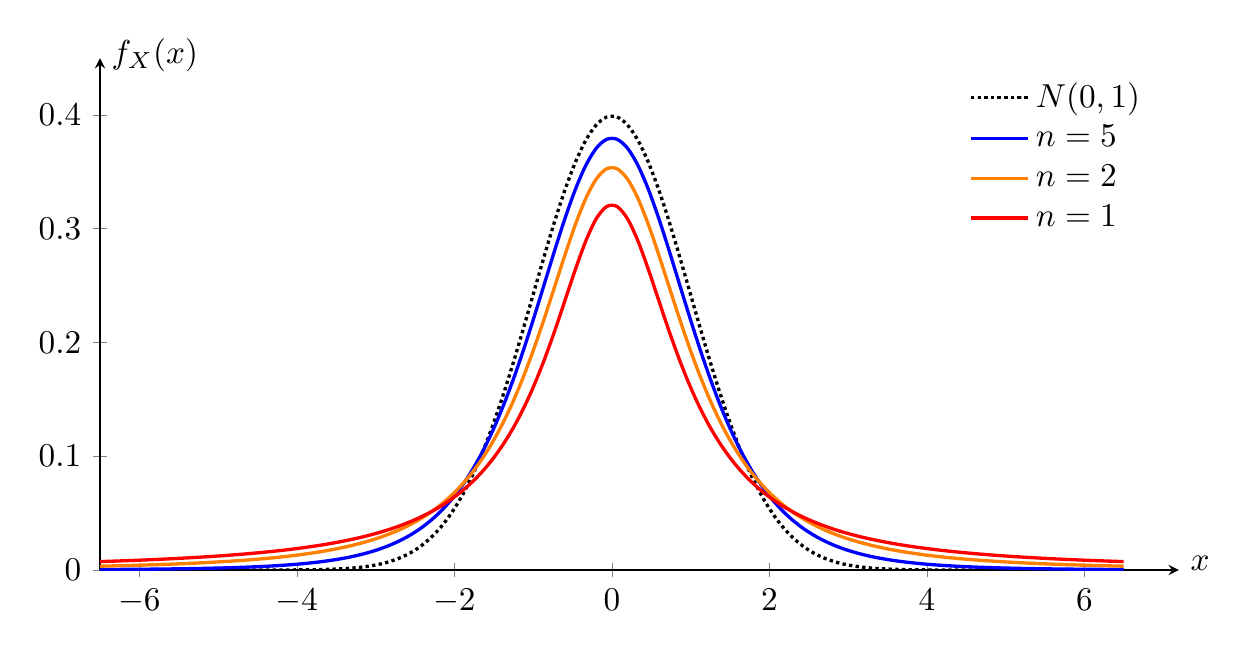
\begin{tikzpicture}[
        declare function={gamma(\z) = 2.506628274631 * sqrt(1/\z) + 0.20888568 * (1/\z)^(1.5) + 0.00870357 * (1/\z)^(2.5) - (174.2106599 * (1/\z)^(3.5))/25920 - (715.6423511 * (1/\z)^(4.5))/1244160) * exp((-ln(1/\z)-1) * \z;},
        declare function={student(\x,\n) = gamma((\n+1)/2)/(sqrt(\n*pi) * gamma(\n/2)) * ((1+(\x*\x)/\n)^(-(\n+1)/2));},
        declare function={normalpdf(\y,\m,\s) = 1/(\s*sqrt(2*pi))*exp(-((\y-\m)^2)/(2*\s^2));},
        scale=1.2
    ]
        \begin{axis}[
            axis lines = left,
            enlargelimits = false,
            samples = 100,
            xmax = 7.2,
            ymax = 0.45,
            xtick = {-6,-4,...,6},
            xlabel = $x$,
            ylabel = $f_X(x)$,
            xlabel style = {at={(rel axis cs:1,0.05)},anchor=north west},
            ylabel style={at={(rel axis cs:0,0.95)},anchor=south west,rotate=-90},
            legend entries = {{$N(0,1)$}, {$n=5$}, {$n=2$}, {$n=1$}},
            legend style = {draw=none},
            legend cell align = left,
            height=7cm,
            width=13cm
        ]
            \addplot [smooth, domain=-6.5:6.5, black, densely dotted, line width=1] {normalpdf(x,0,1)};
            \addplot [smooth, domain=-6.5:6.5, blue, line width=1] {student(x,5)};
            \addplot [smooth, domain=-6.5:6.5, orange, line width=1] {student(x,2)};
            \addplot [smooth, domain=-6.5:6.5, red, line width=1] {student(x,1)};
        \end{axis}
    \end{tikzpicture}
\end{figure}